
\documentclass[12pt, twocolumn]{article}
\usepackage[utf8]{inputenc}
\usepackage{graphicx}

\font\titlefont=cmr12 at 42pt
\title{\vspace{-3.0cm}\titlefont Dreamlands}
\author{Guilherme Oliveira}
\date{}
\pagenumbering{gobble}

\begin{document}

\maketitle

\section*{High Concept}
\paragraph{Fight monsters while stuck in a nightmare, hoping that someday you will truly wake up.}

\paragraph{Everything look cryptic and horror-ish, like everything is a bad \emph{Lovecraftian} dream.}

\section*{Gameplay}

\begin{center}
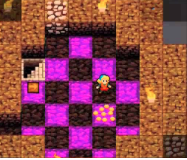
\includegraphics[width=6cm]{images/crypt.png}
\end{center}

\paragraph{Dreamlands has a classical roguelike turn based gameplay, a good reference is Crypt of Necrodancer without the rythim. Engaging in combat happens by moving to the same tile the enemy is on.}

\paragraph{The dungeon is based on The Legend of Zelda and Binding of Isaac, where they are square-ish rooms and you can transition between them.}

\section*{Aesthetics}

\paragraph{Dreamlands is going to be a Pixel Art game with colors that resemble Lovecraftian horror, that means dark and dry colors.}

\paragraph{Concept Art should be more on the cartoony side, good reference can be \emph{Necrodancer} and \emph{Celeste} }

\section*{Why It Needs to Be Made}

\paragraph{This game features an interesting take on the Roguelike genre as it uses a classical input and features used on recent games. Also, it's innovative on the point that it can be played on mobile and can introduce new people to the genre.}

\paragraph{High replayability and a \emph{differential} could be an exponencial difficult increase. Resulting in a faster game loop.}

\section*{Final Thoughts}

\paragraph{Dreamlands can be a beautifully done Turn Based Roguelike that can be on all platforms and bring new people to the genre.}

\end{document}